% A skeleton file for producing Computer Engineering reports
% https://kgcoe-git.rit.edu/jgm6496/KGCOEReport_template

\documentclass[CMPE]{../KGCOEReport}

% The following should be changed to represent your personal information
\newcommand{\classCode}{CMPE 260}  % 4 char code with number
\newcommand{\name}{Andrei Tumbar}
\newcommand{\LabSectionNum}{1}
\newcommand{\LabInstructor}{Moskal}	% The slash is to tell LaTeX that the period is between words
% not sentences so it spaces correctly. It won't appear in the
% final pdf
\newcommand{\TAs}{Jacob Meyerson}
\newcommand{\LectureSectionNum}{2}
\newcommand{\LectureInstructor}{Cliver}
\newcommand{\exerciseNumber}{1}
\newcommand{\exerciseDescription}{Introduction to Vivado \& Simple ALU}
\newcommand{\dateDone}{February 1st}
\newcommand{\dateSubmitted}{February 9th}

\usepackage{tikz}
\usepackage{circuitikz}
\usetikzlibrary{calc}
\usepackage{multirow}
\usepackage{titlesec}
\usepackage{float}
\usepackage{lmodern}
\usepackage{siunitx}
\usepackage{subcaption}
\usepackage{graphicx}
\usepackage[usestackEOL]{stackengine}
\usepackage{scalerel}
\usepackage[T1]{fontenc}
\usepackage{amsmath}

\def\lbar#1{\ThisStyle{%
    \setbox0=\hbox{$\SavedStyle#1$}%
    \stackengine{2.2\LMpt}{$\SavedStyle#1$}{\rule{\wd0}{0.1\LMpt}}{O}{c}{F}{F}{S}%
}}

\DeclareFontFamily{U}{mathx}{\hyphenchar\font45}
\DeclareFontShape{U}{mathx}{m}{n}{ <-> mathx10 }{}
\DeclareSymbolFont{mathx}{U}{mathx}{m}{n}
\DeclareFontSubstitution{U}{mathx}{m}{n}
\DeclareMathAccent{\widebar}{\mathalpha}{mathx}{"73}

\makeatletter
\newcommand{\cwidebar}[2][0]{{\mathpalette\@cwidebar{{#1}{#2}}}}
\newcommand{\@cwidebar}[2]{\@cwideb@r{#1}#2}
\newcommand{\@cwideb@r}[3]{%
    \sbox\z@{$\m@th\mkern-#2mu#3\mkern#2mu$}%
    \widebar{\box\z@}%
}
\newcommand\currentcoordinate{\the\tikz@lastxsaved,\the\tikz@lastysaved}
\makeatother

\newcommand\decbin[9]{%
    \par\smallskip
    \makebox[3cm][r]{$#1$\ }\fbox{#2}\,\fbox{#3}\,\fbox{#4}\,\fbox{#5}\,\fbox{#6}\,\fbox{#7}\,\fbox{#8}\,\fbox{#9}\par}


\def\code#1{\texttt{#1}}

\begin{document}
    \maketitle
    \section*{Abstract}

    In this laboratory exercise, the basics of VHDL were revisited and applied by implementing a simple multi-function ALU.
    The ALU has the ability to apply one of six operations given an input vector.
    \code{OR}, \code{AND}, \code{XOR}, \code{SLL} (Shift-Left-Logical), \code{SRL} (Shift-Right-Logical), and
    \code{SRA} (Shift-Right-Arithmetic).
    These operations are binary operations of N-bit width and could be controlled by the test-bench running the simulation.
    Two sets of test-benches were written to test the ALU in both 4-bit and 32-bit modes.

    \section*{Design Methodology}
    Implementing the 32-bit version of the ALU operations involves providing generic parameters
    to the ALU chip entity.
    The generic parameter can be passed down to child ALU functors such as the SLL, SRL etc circuits.

    A block diagram was created to illustrate the functionality of the ALU operations given a 4-bit operation
    select input.

    \begin{figure}[h!]
        \centering
        %! suppress = Ellipsis
        \begin{circuitikz}[american, ]

            \tikzset{mux16/.style={muxdemux,muxdemux def={Lh=16, NL=16, Rh=14, NB=1, w=3, square pins=0}}}
            \tikzset{aluop/.style={dipchip, num pins=4, hide numbers, no topmark, external pins width=0}}

            % Define the inputs
            \draw (-2.5,1) coordinate(A);
            \draw (-2.5,.5) coordinate(B);
            \draw (A) to[multiwire] ++(-0.5,0) node [anchor=east]{A};
            \draw (B) to[multiwire=N] ++(-0.5,0) node [anchor=east]{B};

            % Generate each of the ALU operations are a dipchip
            \def\Ops{
                % Right side
                OR/0/4,
                AND/0/2,
                XOR/0/0,
                SLL/0/-2,
                SRL/0/-4,
                SRA/0/-6};

            \def\OpPinLength{0.2};
            \def\OpPins{
                % output pin on the right
                out/4/1/left,
                % input pins on the left
                a/1/-1/right,
                b/2/-1/right};

            \foreach \name/\x/\y in \Ops {
                \node [aluop](\name) at (\x,\y) {\name};

                % Generate the input and output pins
                \foreach \subname/\pin/\direction/\labelside in \OpPins {
                    \draw (\name.bpin \pin) -- ++(\OpPinLength*\direction,0) coordinate(\name_\subname);
                    \node [\labelside, font=\tiny] at (\name.bpin \pin) {\subname};
                }
            }

            % Draw the 16 select mux (4 input mux)
            \node [mux16, anchor=lpin 8](ALU) at (4,0){MUX};

            % Label the left pins on the mux in their decimal values
            \foreach \i [evaluate=\i as \pin using int(\i+1)] in {0,...,15} {
                \node [right, font=\tiny] at (ALU.blpin \pin) {\i};
            }

            % Label the select on the mux
            \node [above, font=\tiny] at (ALU.bbpin 1) {op};

            % 3 tuple (CHIP_NAME, BINARY_OPERATOR, MUX_PIN)
            \def\aluinputs{
                 OR/1000/8/0,
                AND/1010/10/0,
                XOR/1011/11/0,
                SLL/1100/12/0,
                SRL/1101/13/-1,
                SRA/1110/14/-3};

            \def\ALUpinspace{-0.2} % spacing between output lins
            \def\ALUpinoffset{-0.3} % offset from the ALU lpin

            \def\OpAoffset{-0.2}
            \def\OpBoffset{-0.6}

            % Pins that are not bound to an operation
            \def\undefinedpins{0,1,2,3,4,5,6,7,9,15}

            % Draw connections from the ALU mux pin to the operators output
            % Also add a label for the binary equivalent value
            \foreach \name/\binlabel/\pin/\spacescale [count=\xi, evaluate=\pin as \pinreal using int(\pin+1)] in \aluinputs {
                \draw (ALU.lpin \pinreal) -- ++(\spacescale*\ALUpinspace + \xi*\ALUpinspace + \ALUpinoffset,0)
                    to [short, *-*] (\currentcoordinate |- \name_out) % go to y-coord for output
                    node[label={[shift={(0,0.3)}, font=\footnotesize] left:\binlabel}] {} % label the wire
                    to[short, *-] (\name_out); % connect to the x-coord

                % Connect the input pins on each operator
                \draw (\name_a) -- ++(\OpAoffset,0) to [short, *-*] (\currentcoordinate |- A) -- (A);
                \draw (\name_b) -- ++(\OpBoffset,0) to [short, *-*] (\currentcoordinate |- B) -- (B);
            }

            % Create a ground to handle undefined select pins
            \draw (ALU.south west) ++(-0.4, -0.2) node[sground](g){};

            % Connect the undefined pins to ground
            \foreach /\pin [count=\xi, evaluate=\pin as \pinreal using int(\pin+1)] in \undefinedpins {
                \draw (ALU.lpin \pinreal) -- (g |- \currentcoordinate) to [short, *-] (g);
            }

            % Connect the OP signal to the mux select
            \draw (ALU.bpin 1) to[multiwire=4] ++(0,-2) node [anchor=north] (OP){OP};

            % Connect the output 'Y' signal to the mux output
            \draw (ALU.rpin 1) to[multiwire=N] ++(2,0) node[anchor=west] (Y){Y};

        \end{circuitikz}
        \caption{Layout of the N-bit ALU with six operations}
        \label{fig:block}
    \end{figure}

    Figure \ref{fig:block} shows a block diagram of the generic-sized input ALU \code{N}.
    The select signal (\code{OP}) is 4 bits long and therefore there are 16 different inputs this signal
    can take.
    The multiplexer in the diagram will handle a subset of the inputs to bind the outputs of valid \code{OP}
    values.
    Figure \ref{fig:block} shows the six valid operations and their corresponding binary values labeled.
    Each operation will take two N-wire signals \code{A} and \code{B}.

    \subsection*{Right-shift design}
    To design the right-shift operations \code{SRL} (logical) and \code{SRA} (arithmetic), a similar approach was
    taken when compared to the \code{SLL} implementation.
    A table of every shift up to \code{N} bits was computed.
    Based on the shift amount \code{B}, a different vector at index \code{B} in the shift table was chosen.
    Shifts above \code{N} will output a \code{0} signal.
    The difference between the arithmetic and logical shifts is the value that the left bits are filled with.
    For a logical shift, the are always 0, for an arithmetic shift, they are equal to the value of the most significant
    bit in the input \code{A}.

    \section*{Results \& Analysis}
    To test the VHDL source code, a test-bench was written to analyse the behaviour of the circuit and all of its
    operations.

    A behavioural waveform was generated.

    \begin{figure}[h!]
        \centering
        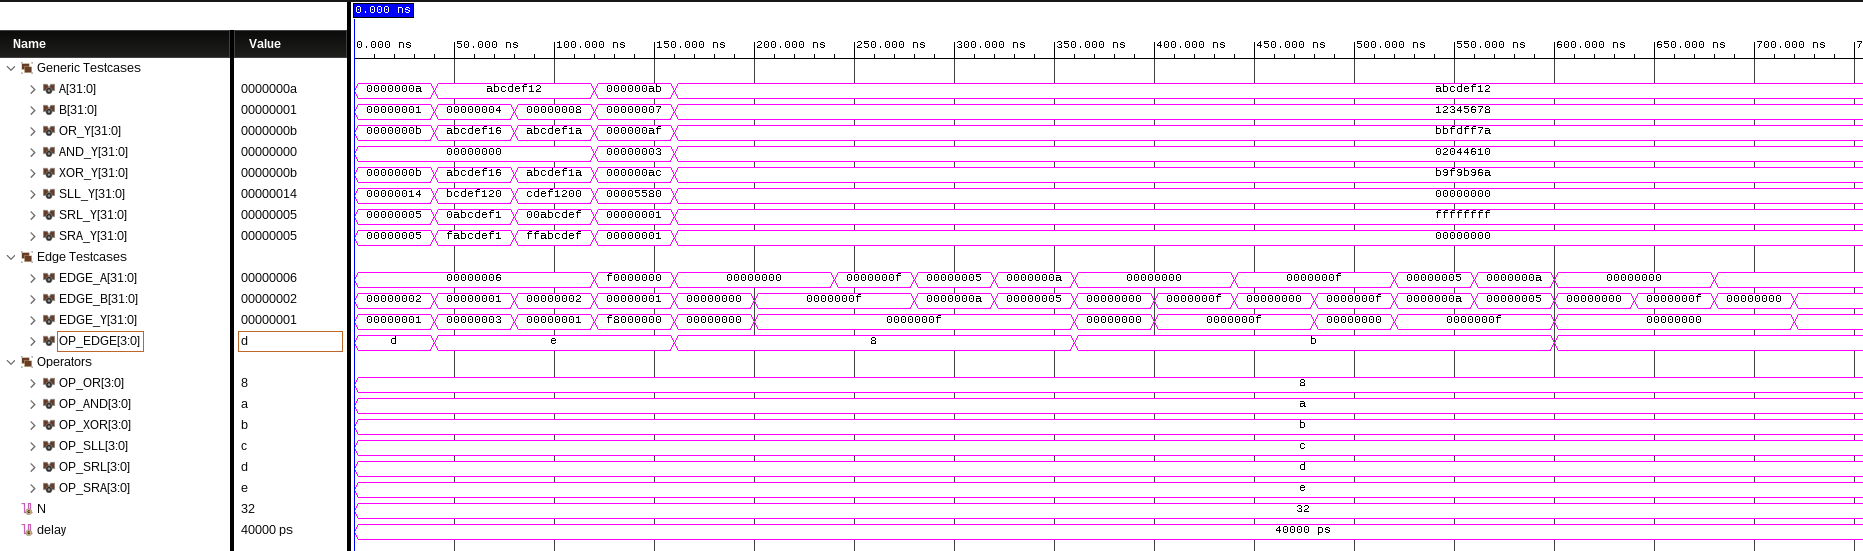
\includegraphics[width=\textwidth]{img/behaviour_32}
        \caption{Screen capture of behavioural simulation in 32-bits}
        \label{fig:behave}
    \end{figure}

    Figure \ref{fig:behave} shows the waveforms generated from running a behavioural simulation of the VHDL
    test-bench.
    All values are denoted in hexadecimal representation for easy readability.
    The signals are split into three sections, Generic Testcases, Edge Testcases, and Operators.
    The operators section are simply constants signal values for each type of operation.
    These are used to understand the \code{OP\_EDGE} signal values.

    The Generic Testcases will test 4 different combinations of inputs \code{A} and \code{B} on all 6
    different ALU operations.
    The output signals simulated in parallel and are named \code{[OP]\_Y} where \code{[OP]} is the ALU operation
    being performed.

    \pagebreak

    Following the behavioural simulation, a Post-Implementation Timing simulation was performed.
    A corresponding waveform was generated.

    \begin{figure}[h!]
        \centering
        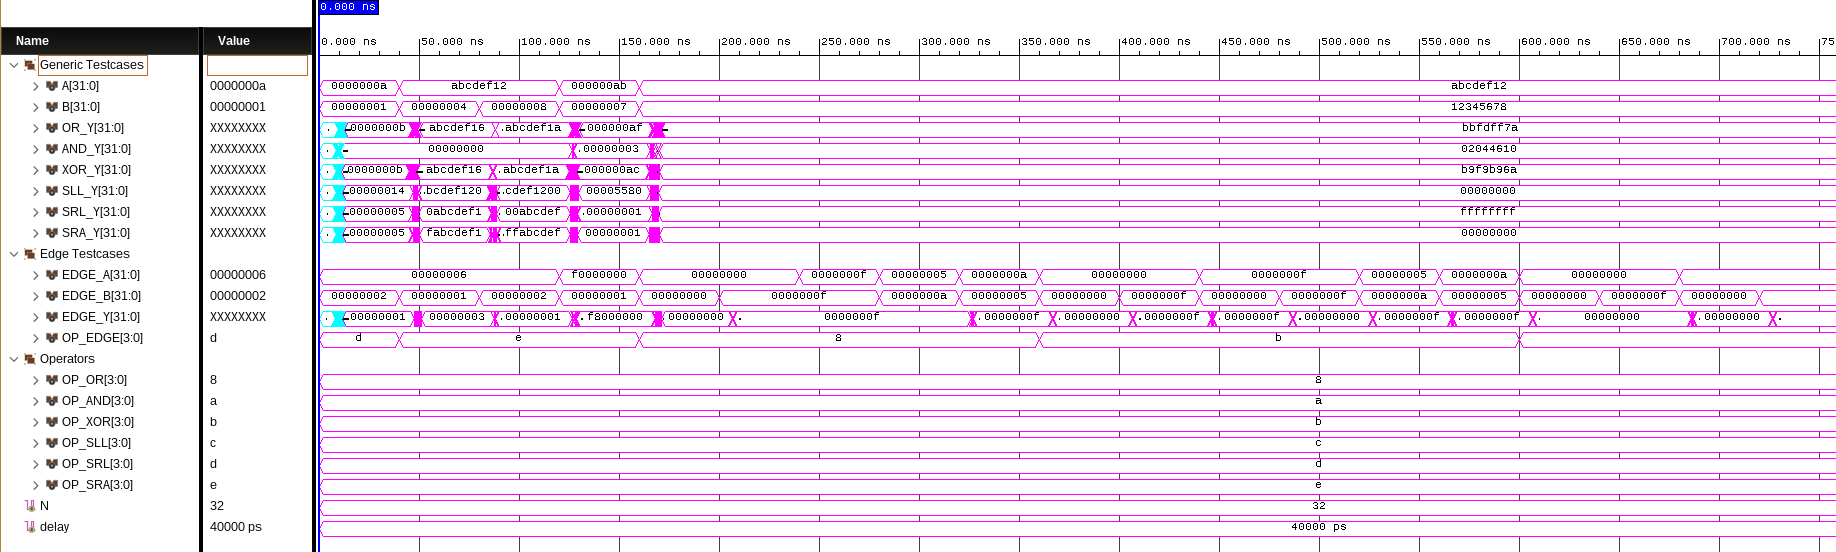
\includegraphics[width=\textwidth]{img/timing_32}
        \caption{Screen capture of timing simulation in 32-bits}
        \label{fig:timing}
    \end{figure}

    The simulation test-bench is identical to the one shown in Figure \ref{fig:behave}.
    In this simulation, the gate delays associated with the Baysis 3 FPGA were taken into account.
    The output signals are seen to change values several nano-seconds after the inputs change.



\end{document}